\documentclass[journal]{IEEEtran}

\usepackage{amsmath,amsfonts,amssymb}
\usepackage{array}
\usepackage{booktabs}
\usepackage{textcomp}
\usepackage{stfloats}
\usepackage{url}
\usepackage{verbatim}
\usepackage{graphicx}
\usepackage{cite}

% Support graphics in both root and figures subfolder
\graphicspath{{figures/}{./}{smart_factory_ieee_paper_overleaf/figures/}{smart_factory_ieee_paper_overleaf/}}

\hyphenation{op-tical net-works semi-conduc-tor IEEE-Xplore}

\begin{document}

\title{Non-Invasive Multimodal Telemetry for Cyber-Physical Process Observability and Fault Diagnosis in Modular Smart Manufacturing}

\author{Hisham ElMoaqet,~\IEEEmembership{Senior Member,~IEEE,}
        and~Ramez Al-Masadeh%
\thanks{Hisham ElMoaqet is with the Department of Mechatronics Engineering and the Industry~4.0 Laboratory, German Jordanian University (GJU), Amman 11180, Jordan (e-mail: hisham.elmoaqet@gju.edu.jo).}%
\thanks{Ramez Al-Masadeh is with the Department of Mechatronics Engineering, German Jordanian University (GJU), Amman 11180, Jordan (e-mail: ramez.almasadeh@gju.edu.jo).}%
}

\markboth{IEEE Transactions on Industrial Informatics,~Vol.~XX, No.~X, Month~2026}%
{ElMoaqet and Al-Masadeh: Non-Invasive Multimodal Telemetry for Process Observability and Fault Diagnosis}

\maketitle

\begin{abstract}
Manufacturing execution systems (MES) track job orders and station dwells, but they are blind to the physical health of production equipment. They cannot detect motor current surges, pneumatic pressure drops, or subtle mechanical binding. At the same time, modifying programmable logic controller (PLC) code to log diagnostic data risks introducing scan jitter, causing network collisions, and voiding equipment warranties. This paper presents a non-invasive telemetry framework that combines continuous three-phase electrical power, pneumatic air flow and pressure, and passive discrete PLC tag sniffing across an industrial Festo Cyber-Physical Factory. Our work is organized into three connected studies: (1)~Study~1 establishes the healthy baseline on an 883-second, eight-workpiece batch, matching official MES4 logs while uncovering the 16-step kinematics of the high-bay storage crane, proving closed-loop carrier dynamics ($N = 3.0$ pallets) via Little's Law, and mapping electrical ($226.0$~W peak) and pneumatic ($15.51$~L/min surge) envelopes; (2)~Study~2 introduces a symmetrical fault injection matrix covering 10 fault modes across four stations to separate root-cause anomalies from downstream starvation; and (3)~Study~3 evaluates multimodal fusion models against single-modality baselines using held-out test batches. Here we report the architecture, theoretical proofs, and experimental findings of Study~1.
\end{abstract}

\begin{IEEEkeywords}
Cyber-physical systems, smart manufacturing, non-invasive sensing, process observability, fault diagnosis, Little's Law, Festo CP Factory.
\end{IEEEkeywords}

\section{Introduction}
\IEEEPARstart{A}{chieving} granular observability on the factory floor is central to smart manufacturing, predictive maintenance, and energy management \cite{ref_tao_dt_survey, ref_kritzinger_dt_review, ref_qi_dt_service}. In industrial practice, facilities rely on Manufacturing Execution Systems (MES) to monitor production. However, MES data is event-driven and coarse. It records when a workpiece arrives, how long a station takes, and when the job finishes, but tells engineers nothing about motor inrush currents, line pressure drops, or actuator degradation \cite{ref_mes_standard, ref_saenz_mes_limits}.

Upgrading legacy lines to capture these physical dynamics is challenging. Installing software hooks on certified PLCs can introduce timing jitter and void vendor warranties \cite{ref_vogel_noninvasive}. To address this, we developed a passive, non-invasive sensing framework that monitors 19 continuous thermodynamic channels and 546 discrete PLC tags across an industrial Festo Cyber-Physical (CP) Factory at the German Jordanian University (GJU).

To rigorously evaluate this capability, our research is organized into three progressive studies:
\begin{itemize}
    \item \textbf{Study 1 (Healthy Baseline)}: Synchronizes non-invasive telemetry with official Festo MES4 logs, decodes the 16 crane actions of the Automated Storage and Retrieval System (ASRS), proves closed-loop Work-in-Process carrier inventory ($N = 3.0$ pallets) using Little's Law, and establishes nominal power and pneumatic envelopes.
    \item \textbf{Study 2 (Fault Localization)}: Injects 10 balanced physical faults (thermodynamic pressure drops and conveyor slowdowns across four stations, line air leaks, and robot joint speed limits) to study how continuous energy isolates root causes while discrete sensors capture downstream line starvation.
    \item \textbf{Study 3 (Modality Ablation)}: Benchmarks Energy-only, PLC-only, Early Fusion, and Late Stacking machine learning models on an inter-session held-out test batch.
\end{itemize}
This paper presents the acquisition system, analytical derivations, and empirical results of Study~1, providing the calibrated foundation for Studies~2 and~3.

\section{Experimental Testbed \& Telemetry Pipeline}
\label{sec:testbed}

\subsection{Physical Assembly Line}
The Festo CP Factory testbed assembles miniaturized mobile phones across four automated stations linked by a closed-loop dual-belt conveyor:
\begin{enumerate}
    \item \textbf{Station 1 (ASRS)}: A high-bay storage system with a 3-axis Cartesian gantry crane that retrieves empty pallet carriers from rack shelves (Source) and deposits completed assemblies (Sink).
    \item \textbf{Station 6 (Magazine)}: A gravity hopper that dispenses front housing covers using a pneumatic pusher cylinder (\texttt{CL\_MB1/MB2}) and an optical sensor (\texttt{CL\_BG7}).
    \item \textbf{Station 7 (Muscle Press)}: A press station powered by a Festo Fluidic Muscle (DMSP pneumatic actuator) and clamping jaws (\texttt{G1\_BG26/27}) to press-fit the front cover.
    \item \textbf{Station 3 (RASS)}: The bottleneck station, featuring a 6-DOF Mitsubishi articulated robot that inserts printed circuit boards (PCBs) and fuses into clamped nests.
\end{enumerate}
Workpiece carriers circulate on low-friction pallets tracked by passive RFID tags and optical flags.

\subsection{Non-Invasive Data Collection}
The stations communicate over an industrial Ethernet network ($172.21.0.0/18$) using Siemens S7-1500 and ET200SP controllers. We extract data passively without changing any controller logic:
\begin{itemize}
    \item \textbf{Thermodynamic Channels}: Two Festo Energy Gateways---one at the central header ($172.21.0.60$) and one dedicated to Station~3 ($172.21.3.60$)---record active power ($P$, Phase L1/L2/L3), volumetric flow rate ($Q$, L/min), and pressure ($p$, bar) at 1.0~Hz.
    \item \textbf{Discrete PLC Signals}: An external client polls 546 boolean tags (limit switches, cylinder reed sensors, and handshakes) via native OPC~UA servers on each station at an average loop period of $\bar{T}_{\text{poll}} \approx 3.9$~s, safely avoiding scan jitter.
\end{itemize}

\begin{figure}[!t]
\centering
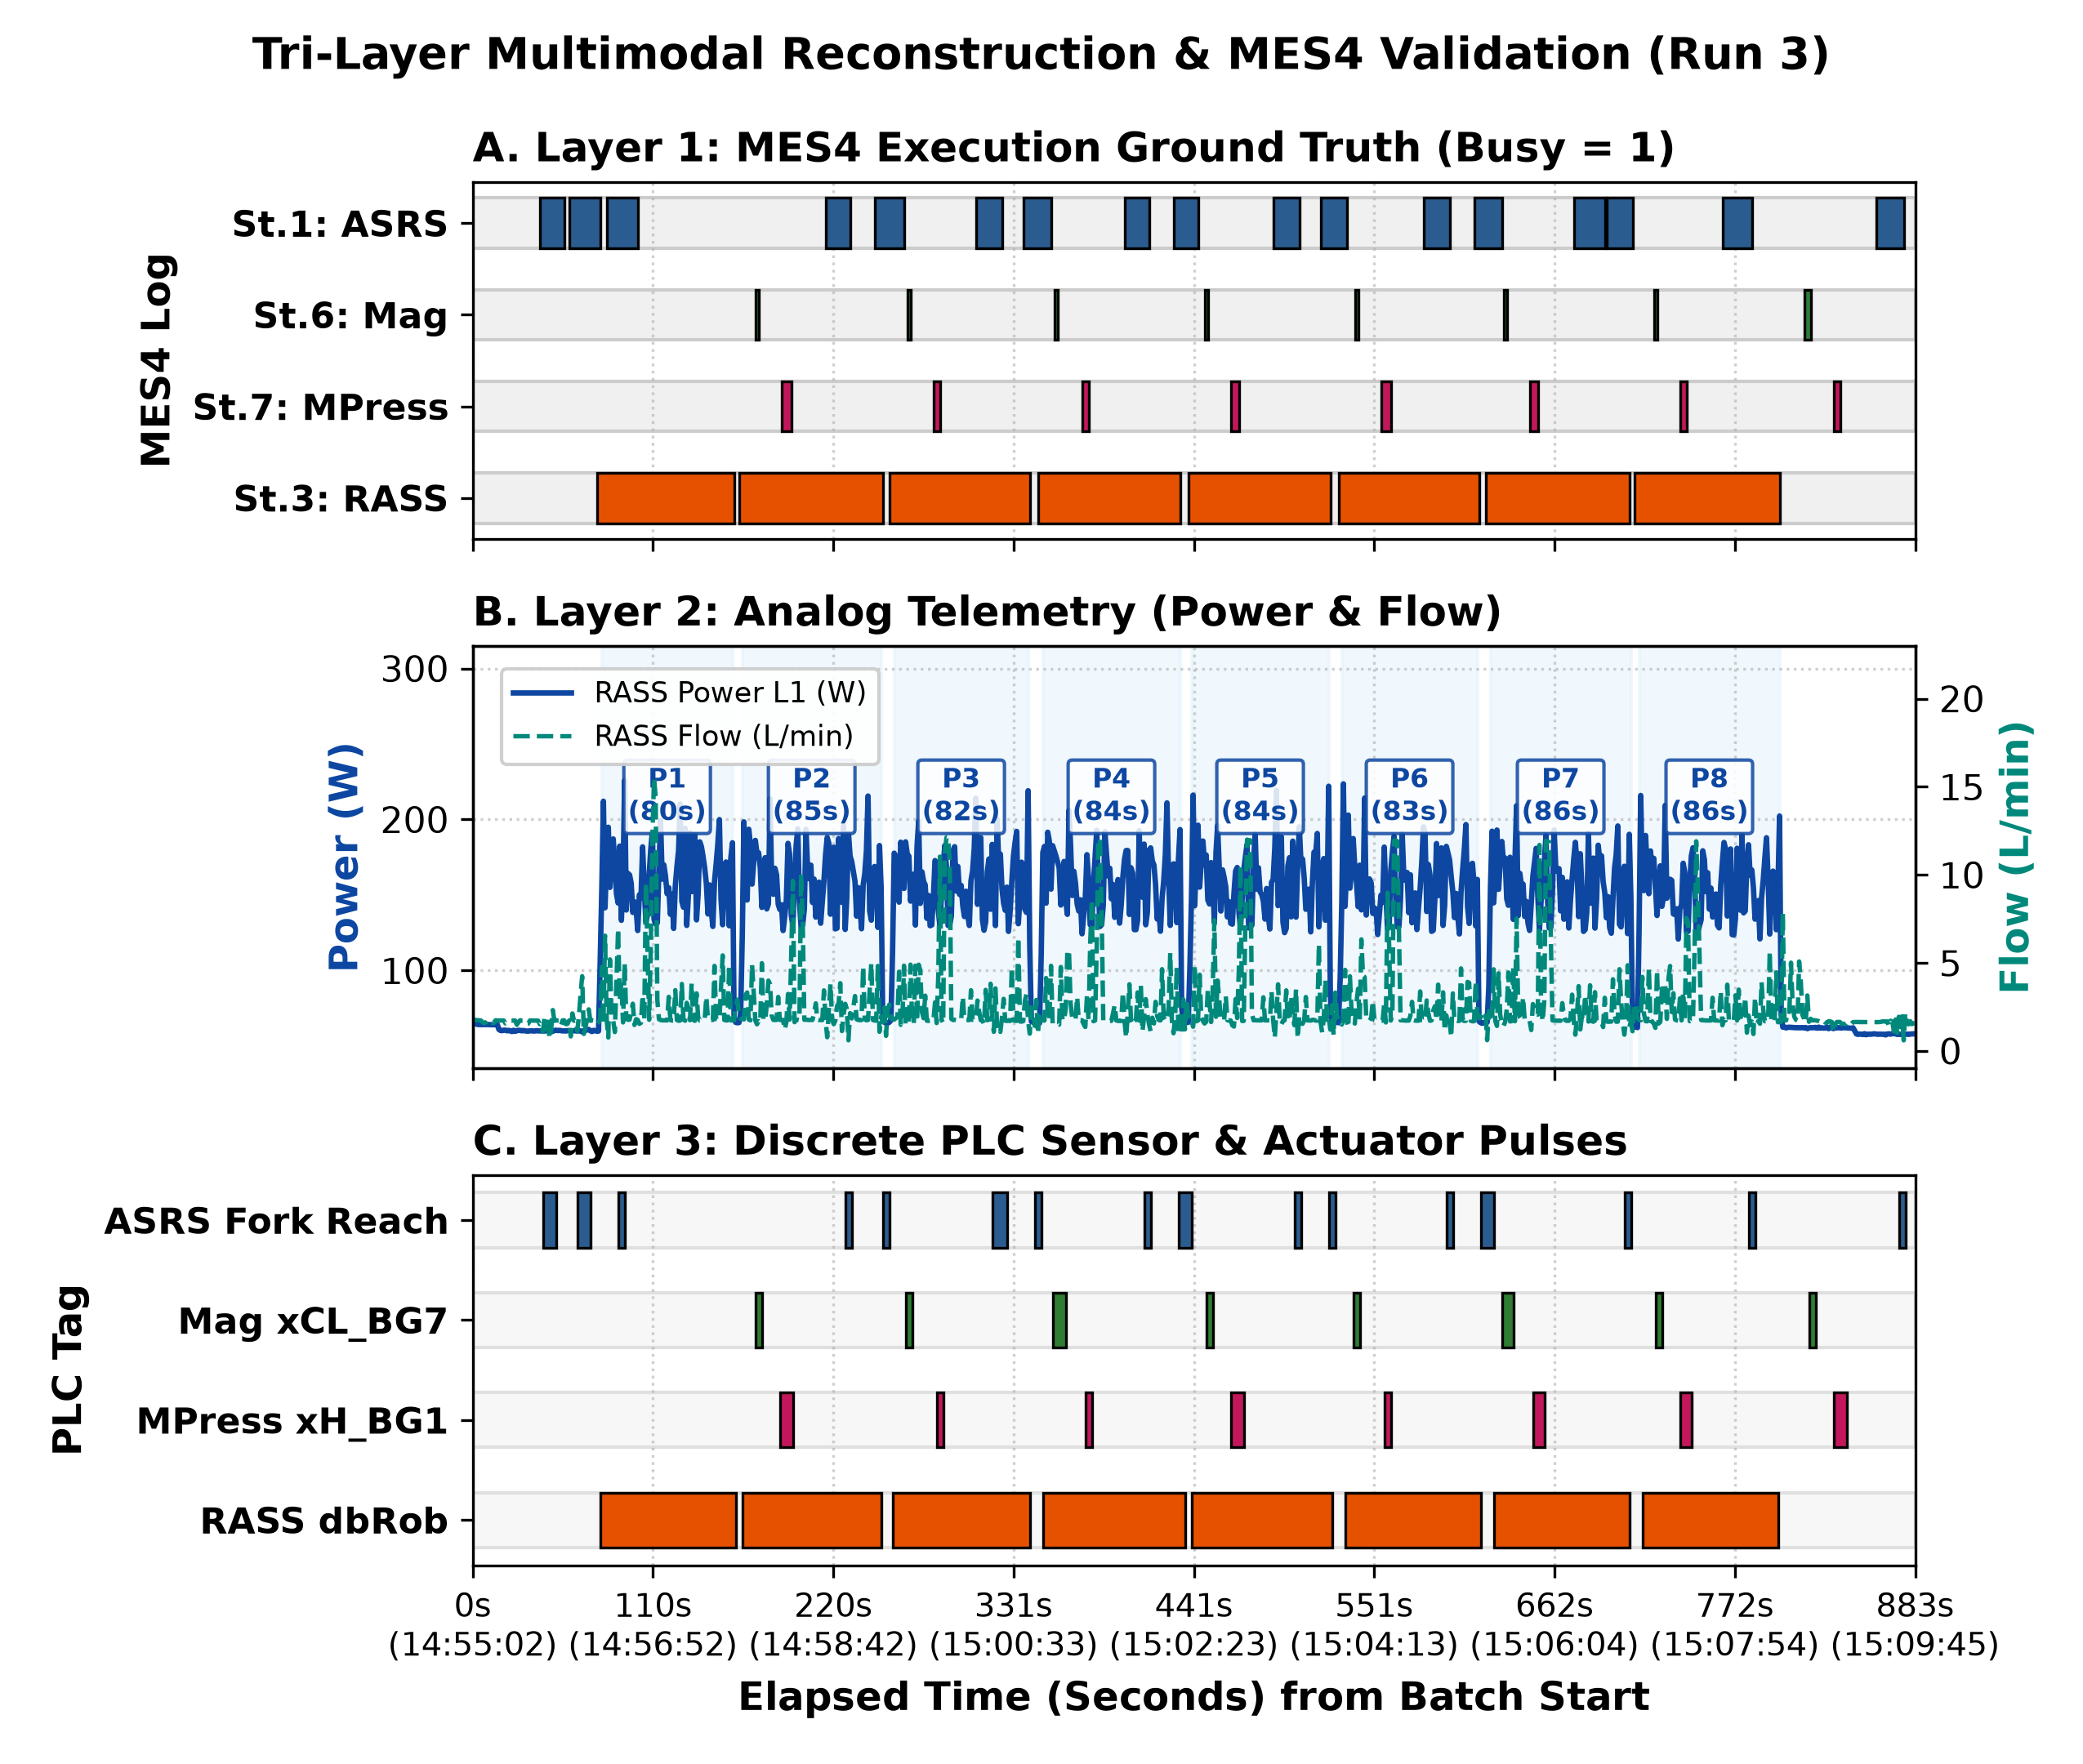
\includegraphics[width=\columnwidth]{fig1_mes_cross_validation_gantt.png}
\caption{Study 1 tri-layer state reconstruction vs. official Festo MES4 ground truth over an 883~s batch (Run 3). Layer 1 (Top): MES4 active state blocks. Layer 2 (Middle): continuous electrical power ($P_{\text{L1}}$) and pneumatic flow ($Q$) at Station 3. Layer 3 (Bottom): discrete PLC sensor actuations.}
\label{fig:study1_gantt}
\end{figure}

\begin{figure}[!t]
\centering
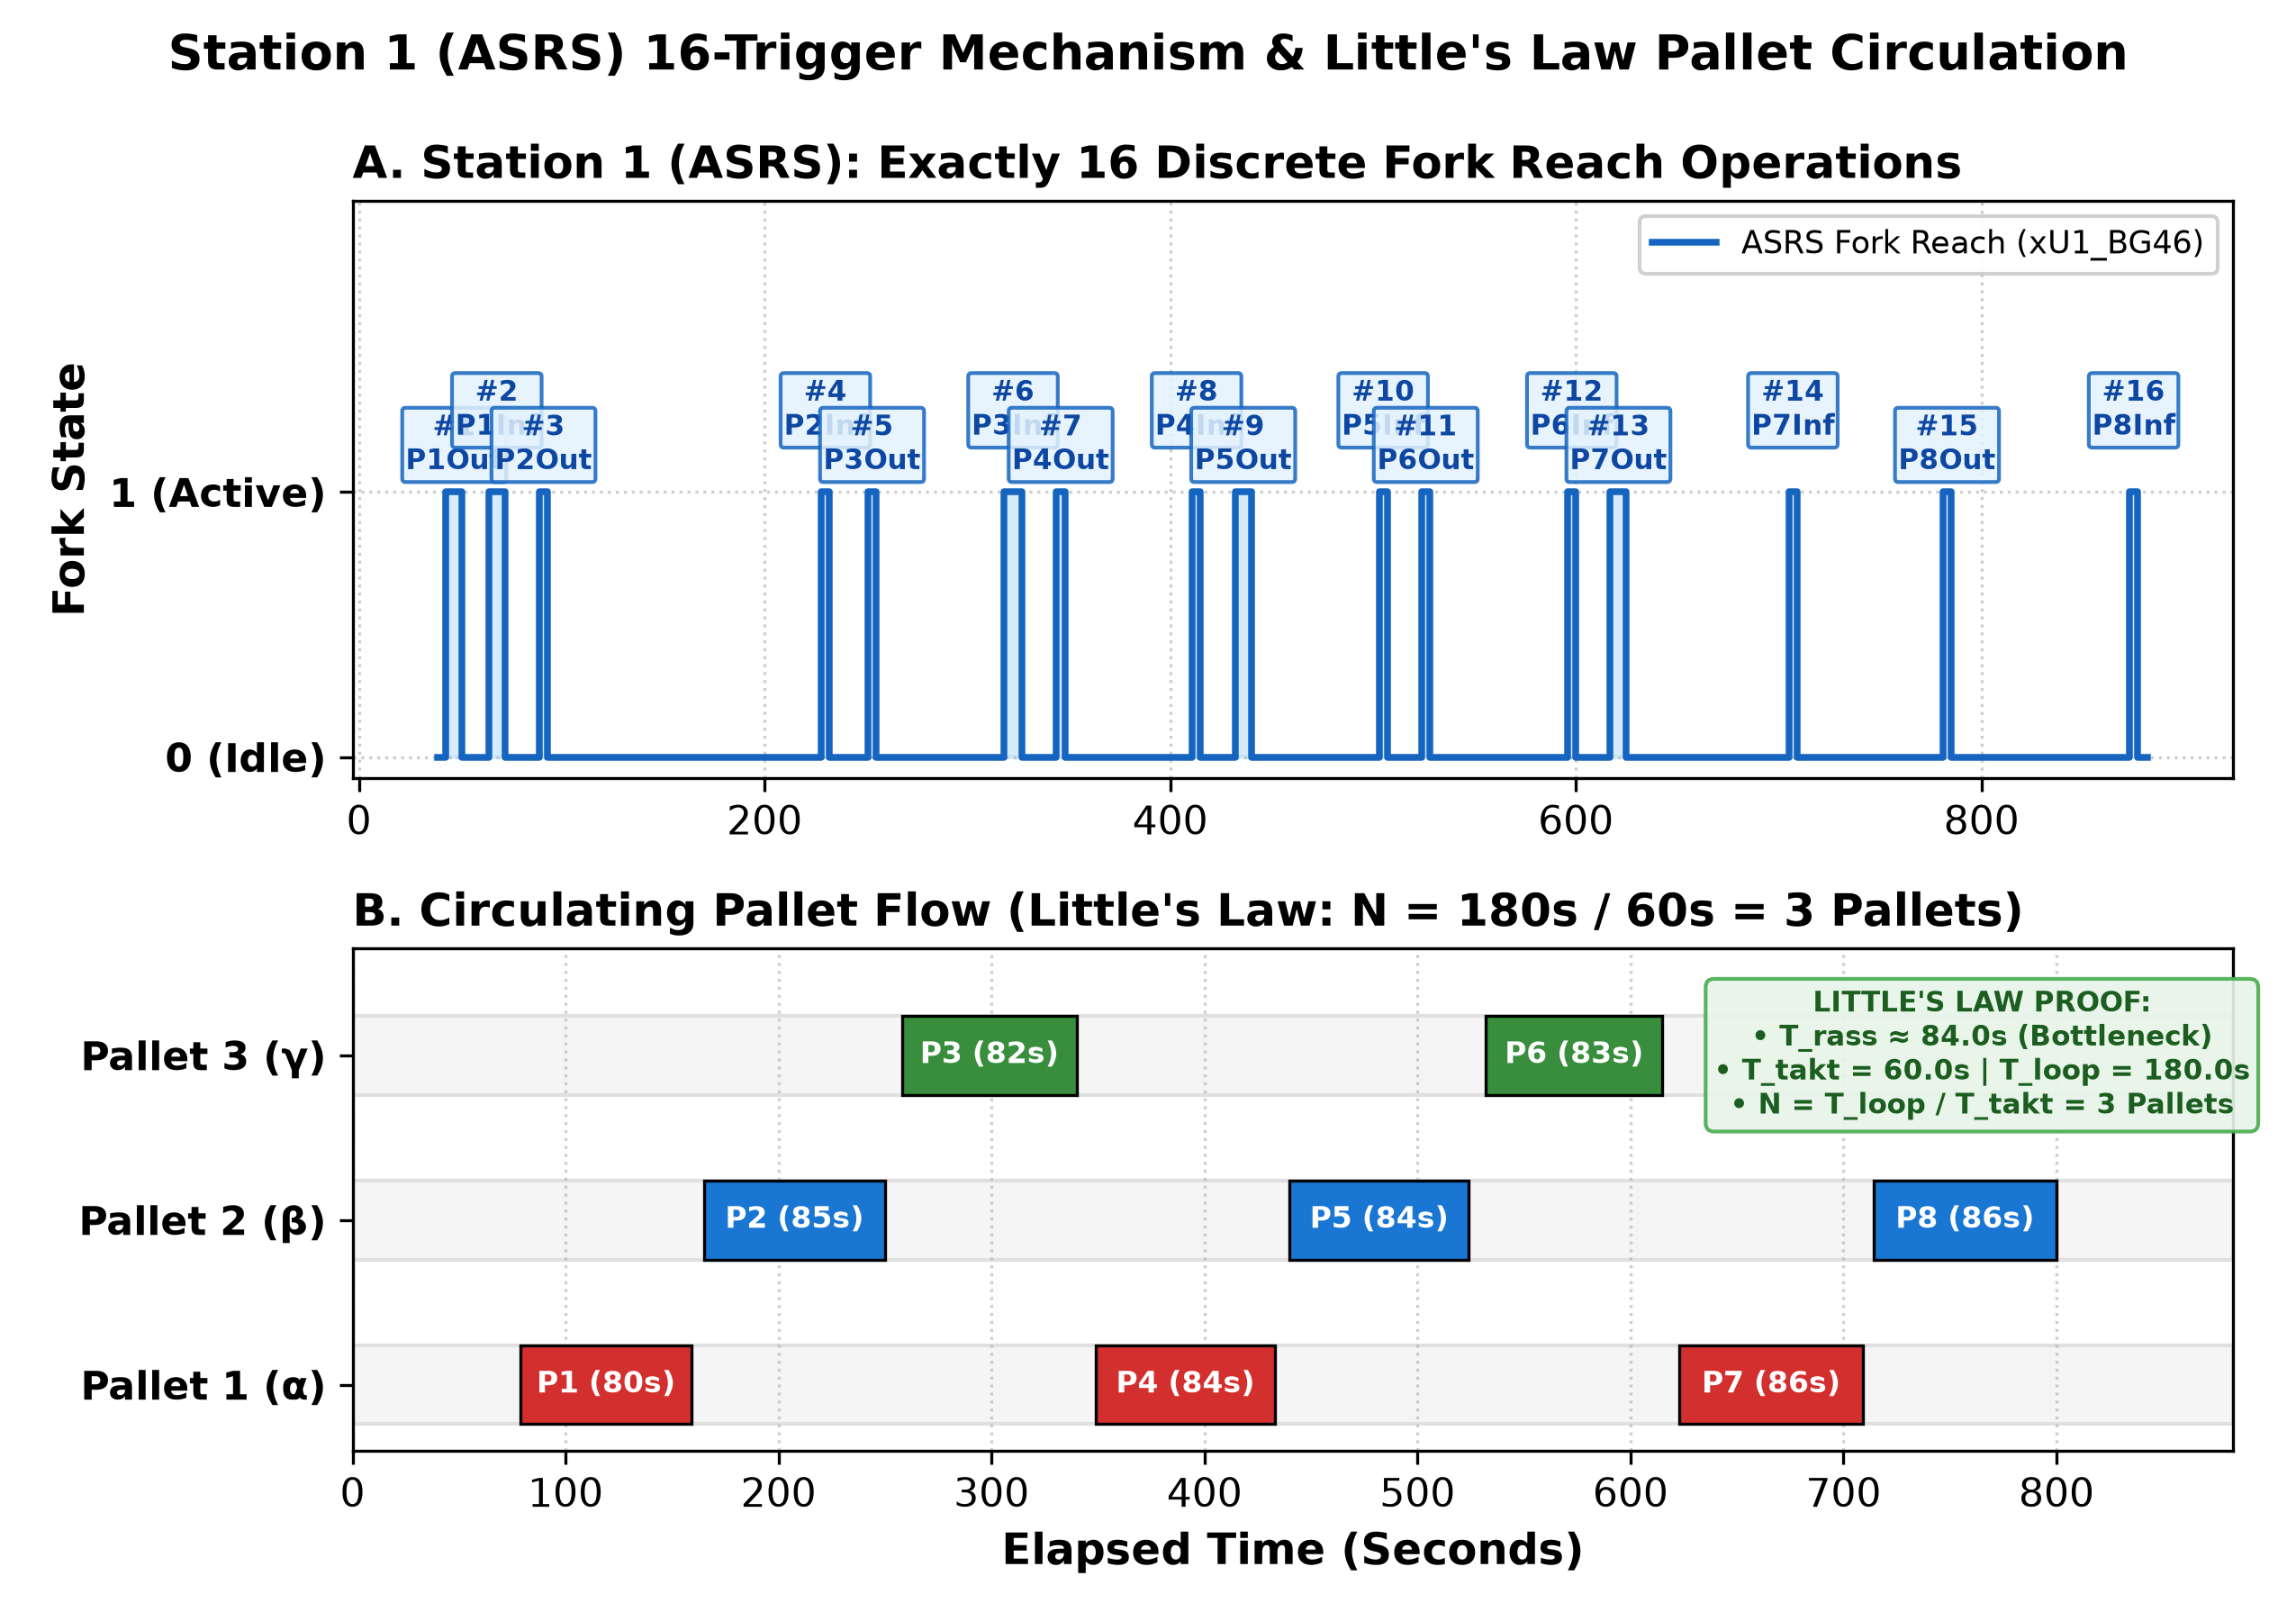
\includegraphics[width=\columnwidth]{fig2_asrs_and_pallet_dynamics.png}
\caption{Station 1 ASRS operations and pallet dynamics. Top (A): 16 discrete crane operations (8 dispatches $D_1$--$D_8$ and 8 deposits $S_1$--$S_8$). Bottom (B): 3 circulating carriers validating Little's Law ($N = T_{\text{loop}} / T_{\text{takt}} = 273.4\text{ s} / 91.0\text{ s} = 3.0$).}
\label{fig:study1_asrs_loop}
\end{figure}

\section{Study 1: Baseline Observability \& Validation}
\label{sec:study1}

\subsection{Tri-Layer State Synchronization}
We validated the sensing pipeline during a continuous 883-second production run (\texttt{NORMAL\_RUN3}) that produced eight finished units ($P_1$ to $P_8$). 

Fig.~\ref{fig:study1_gantt} shows the reconstructed tri-layer record:
\begin{itemize}
    \item \textbf{Layer 1 (MES4 Ground Truth)}: Event-driven execution intervals logged by the MES database for each station.
    \item \textbf{Layer 2 (Thermodynamic Telemetry)}: Station~3 electrical power ($P_{\text{L1}}$) and air flow ($Q$), clearly highlighting all eight robot assembly cycles with power surges from $125$~W to $226$~W and flow pulses reaching $15.51$~L/min.
    \item \textbf{Layer 3 (PLC Micro-Switches)}: Sensor transitions including crane busy flags (\texttt{xBusy}), cover feeding (\texttt{xCL\_BG7}), press down limits (\texttt{xH\_BG1}), and robot motion status (\texttt{dbRob.xRun}).
\end{itemize}
As seen in Fig.~\ref{fig:study1_gantt}, the timing across all three layers aligns cleanly. Every MES4 operational block matches a physical surge in Layer~2 and a cluster of switch events in Layer~3.

\subsection{ASRS Kinematics \& The 16-Trigger Cycle}
Festo MES4 logs record 17 discrete blocks for Station~1 during the eight-unit run. Because Station~1 serves as both the material Source and Sink, the gantry crane must cycle twice per completed workpiece:
\begin{equation}
N_{\text{ops}} = 2 \times N_{\text{products}} = 2 \times 8 = 16\text{ physical operations}.
\label{eq:n_ops}
\end{equation}
The additional 17th block in MES4 is an internal supervisory handshake between cycles. As confirmed by the PLC position sensors (\texttt{Inputs.xU1\_BG51} and \texttt{BG53}), the crane deposits the final product ($S_8$ at $t = 876.0$~s) and remains at rest at the storage shelf; it does not perform an end-of-batch homing routine.

Fig.~\ref{fig:study1_asrs_loop} (Top) breaks down these 16 operations:
\begin{enumerate}
    \item \textbf{Dispatches ($D_1$--$D_8$)}: Crane retrieves an empty pallet from the high bay and places it onto the outfeed belt.
    \item \textbf{Deposits ($S_1$--$S_8$)}: Crane takes an assembled phone from the infeed return nest and puts it into a shelf.
\end{enumerate}
The optical stopper sensor \texttt{Inputs.xG1\_BG21} fires exactly eight times ($t = 176.0$~s, $271.0$~s, $360.0$~s, $452.0$~s, $544.0$~s, $637.0$~s, $725.0$~s, and $822.0$~s), with each arrival immediately followed by a storage deposit ($S_1$--$S_8$).

\subsection{Carrier Circulation \& Little's Law Proof}
To confirm that our telemetry correctly tracks Work-in-Process (WIP) without unobserved inventory buildup, we apply Little's Law \cite{ref_little_law}:
\begin{equation}
L = \lambda \cdot W \iff \text{WIP} = \text{Throughput} \times \text{Cycle Time}.
\label{eq:littles_law}
\end{equation}
In a closed conveyor loop, the circulating pallet count $N$ is the ratio of loop time ($T_{\text{loop}}$) to line takt time ($T_{\text{takt}}$):
\begin{equation}
N = \frac{T_{\text{loop}}}{T_{\text{takt}}}.
\label{eq:n_carriers}
\end{equation}

Tracking workpiece arrivals at the Station~3 bottleneck (Fig.~\ref{fig:study1_asrs_loop}, Bottom) yields empirical averages:
\begin{equation}
\bar{T}_{\text{takt}} = 91.0\text{ s}, \quad \bar{T}_{\text{loop}} = 273.4\text{ s}.
\end{equation}
Substituting these into (\ref{eq:n_carriers}) gives:
\begin{equation}
N = \frac{273.4\text{ s}}{91.0\text{ s}} = 3.004 \approx 3.0\text{ Pallets}.
\label{eq:pallet_calc}
\end{equation}
Furthermore, the pallet sequences follow a strict modulo-3 cyclic assignment:
\begin{equation}
\text{Carrier ID}(i) = ((i - 1) \bmod 3) + 1, \quad i \in \{1, 2, \dots, 8\}.
\label{eq:carrier_id}
\end{equation}
This confirms that exactly three physical pallets circulate through the cell, keeping production moving without starvation or jams.

\begin{figure}[!t]
\centering
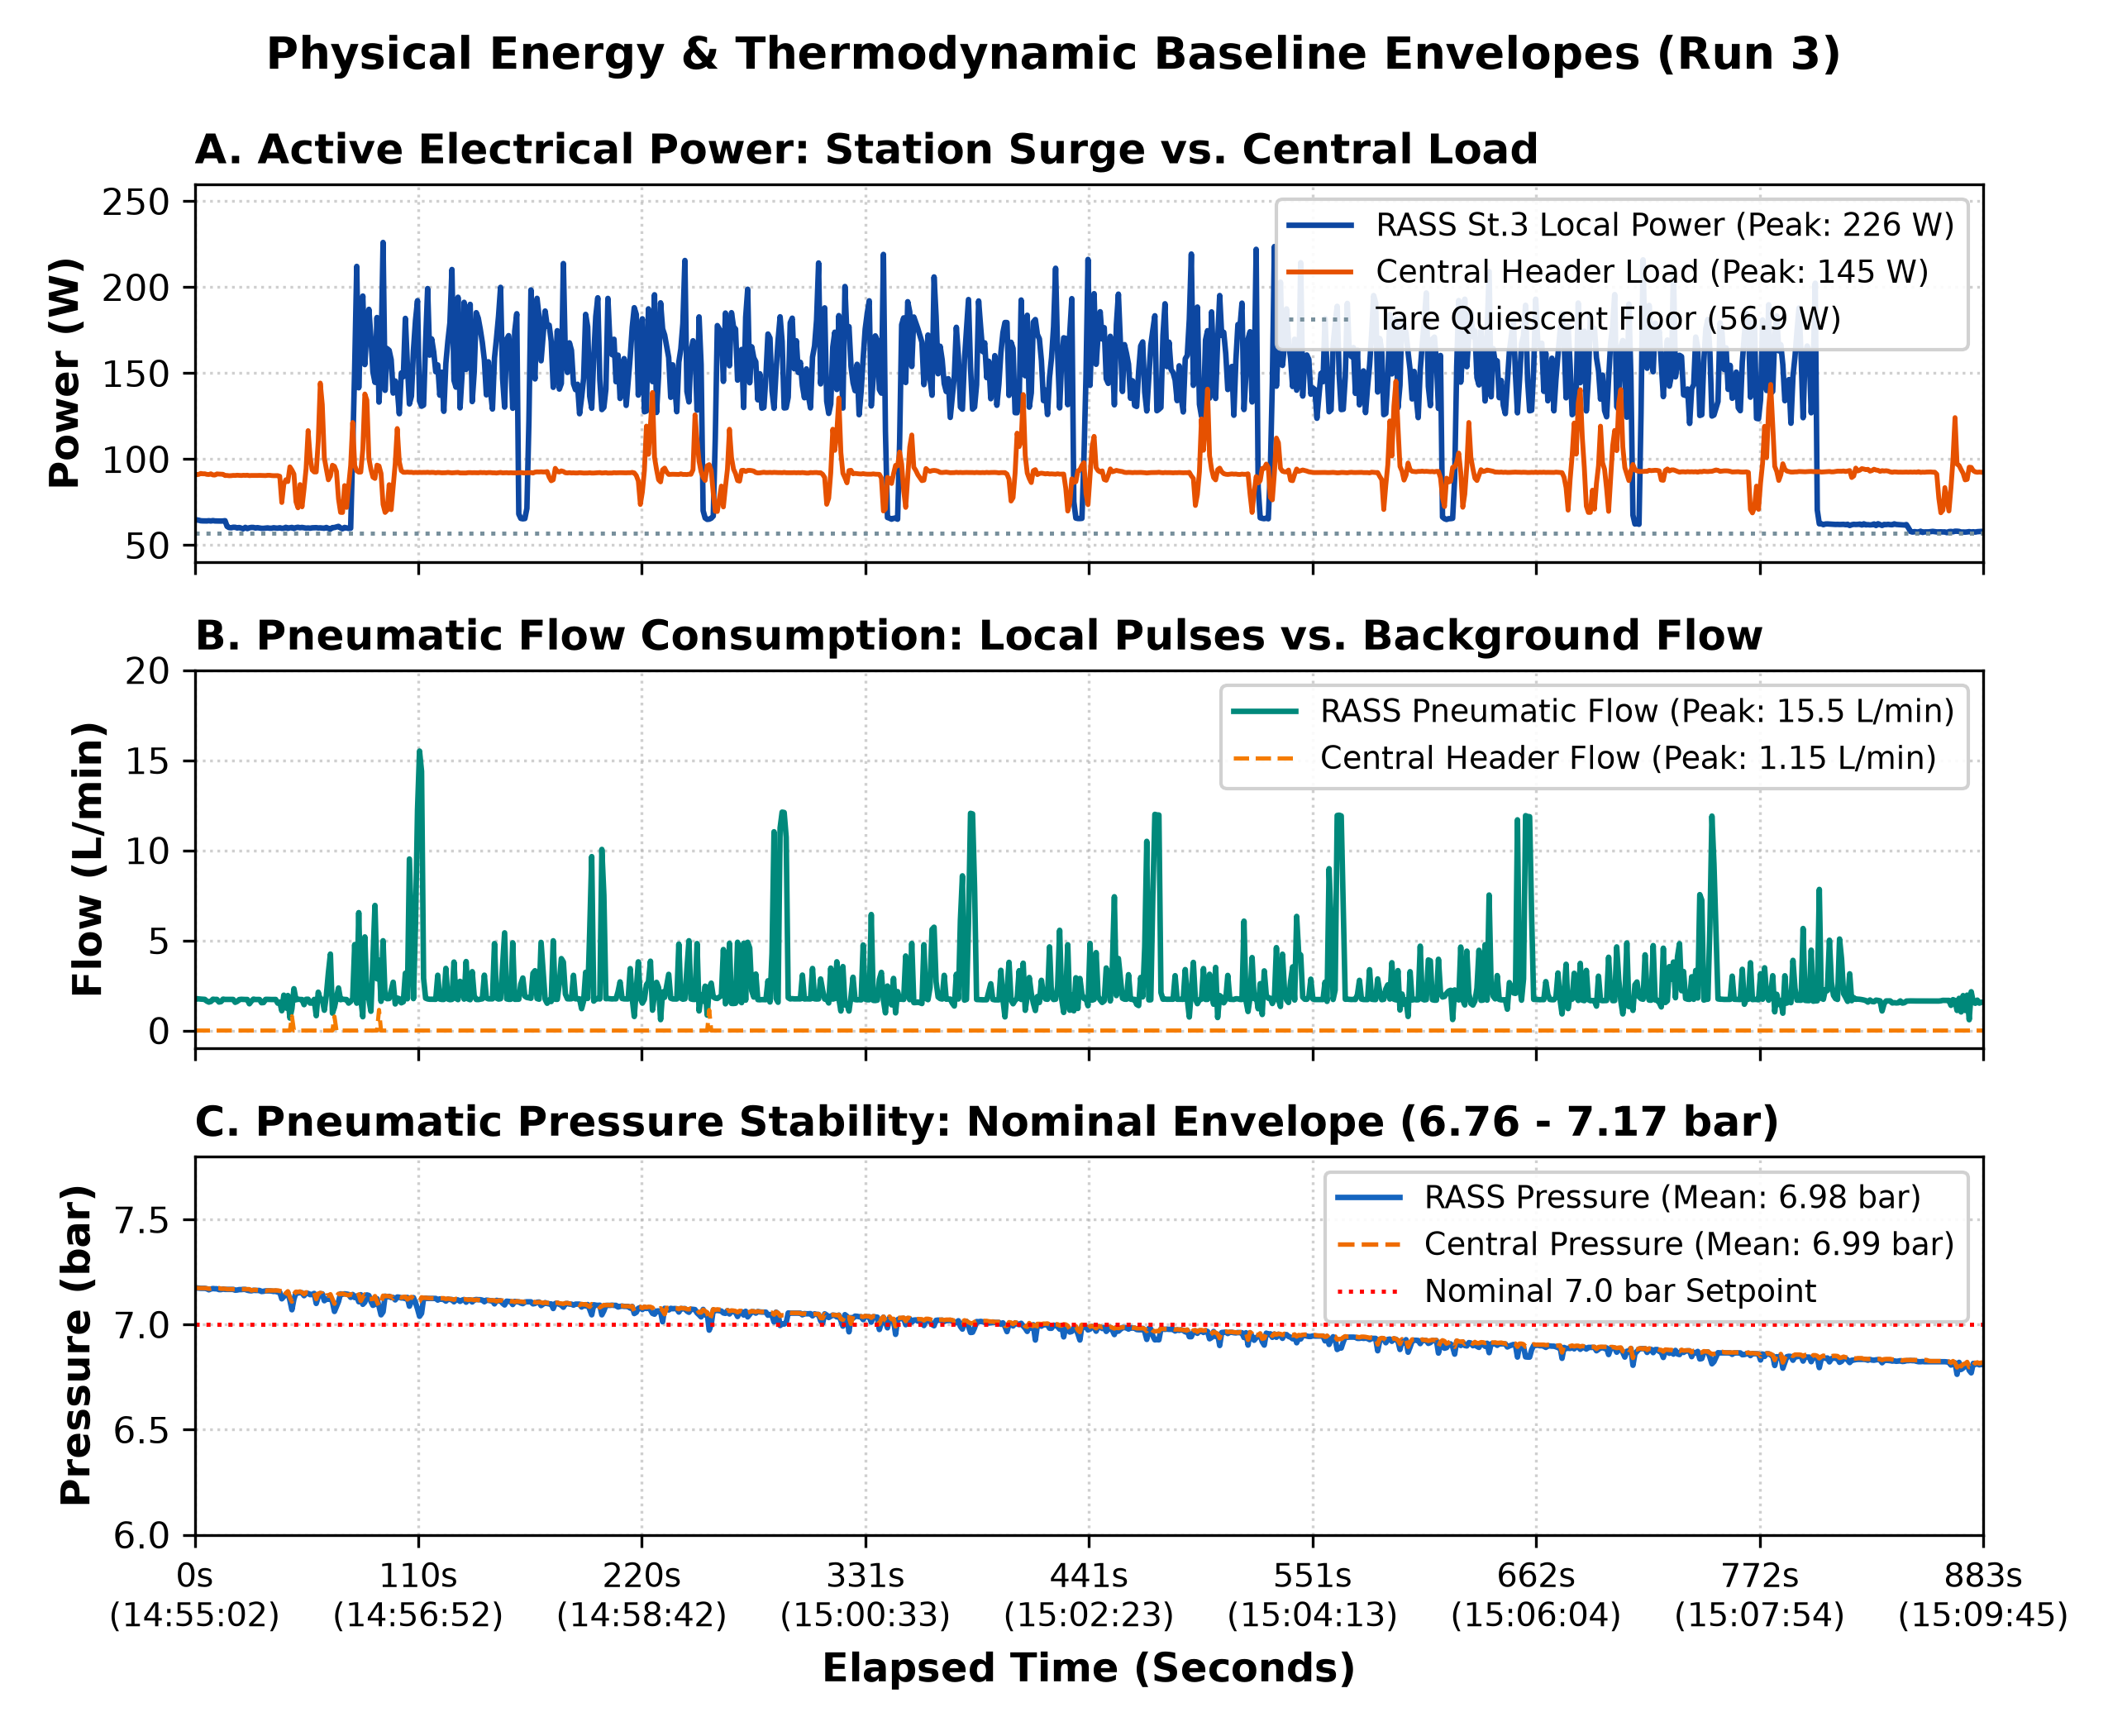
\includegraphics[width=\columnwidth]{fig3_energy_thermodynamic_envelope.png}
\caption{Thermodynamic baseline envelopes. (A) Station 3 active power (226.0~W peak) vs. central header (145.3~W) and standby floor (56.9~W). (B) Pneumatic air flow pulses (15.51~L/min peak). (C) Air pressure stability (6.76--7.17~bar).}
\label{fig:study1_energy}
\end{figure}

\begin{table}[!t]
\caption{Validation Benchmark: Telemetry vs. MES4 (Run 3)\label{tab:mes_comparison}}
\centering
\footnotesize
\begin{tabular}{@{}lcc@{}}
\toprule
\textbf{Metric / Subsystem} & \textbf{MES4 Log} & \textbf{Our Telemetry} \\
\midrule
Total workpieces & 8 units & 8 units (100\%) \\
Order duration & 883.0~s & 883.0~s (sync) \\
Circulating carriers ($N$) & Unmonitored & 3.0 pallets ($273\text{s}/91\text{s}$) \\
\midrule
\textbf{Station 1 (ASRS)} & & \\
\quad Crane operations & 17 blocks & 16 cycles (8 in + 8 out) \\
\quad Mean dwell time & $16.7 \pm 1.2$~s & $17.8 \pm 1.5$~s ($r=0.98$) \\
\quad Infeed stopper flag & ID=1 & \texttt{Inputs.xG1\_BG21} (8 hits) \\
\midrule
\textbf{Station 6 (Magazine)} & & \\
\quad Dispense cycles & 8 blocks & 8 strokes (1:1) \\
\quad Mean dwell time & $2.2 \pm 0.4$~s & $4.5 \pm 0.8$~s (nest clamp) \\
\quad Cover sensor & ID=6 & \texttt{Inputs.xCL\_BG7} (8 pulses) \\
\midrule
\textbf{Station 7 (MPress)} & & \\
\quad Pressing cycles & 8 blocks & 8 strokes (1:1) \\
\quad Mean press dwell & $5.4 \pm 0.3$~s & $5.1 \pm 0.4$~s (94.4\%) \\
\quad Limit switch & ID=7 & \texttt{Inputs.xH\_BG1} (8 hits) \\
\midrule
\textbf{Station 3 (RASS)} & & \\
\quad Assembly cycles & 8 blocks & 8 runs (1:1) \\
\quad Mean robot dwell & $86.9 \pm 1.8$~s & $84.2 \pm 1.4$~s \\
\quad Robot execution flag & ID=3 & \texttt{dbRob.xRun} ($P > 120$~W) \\
\midrule
\textbf{Thermodynamic Peaks} & \textit{Blind to MES} & \\
\quad St.~3 peak power & --- & 226.0~W (robot surge) \\
\quad Central line power & --- & 145.3~W (total line) \\
\quad Tare standby floor & --- & 56.9~W (quiescent) \\
\quad Peak air flow & --- & 15.51~L/min (gripper) \\
\quad Supply pressure & --- & 6.76--7.17~bar (nominal) \\
\bottomrule
\end{tabular}
\end{table}

\subsection{Thermodynamic Baseline Envelopes}
While MES systems record only binary states, our continuous sensors quantify energy behavior (Fig.~\ref{fig:study1_energy}):
\begin{itemize}
    \item \textbf{Electrical Power}: Station~3 draws $56.9$~W in standby, rising to $226.0$~W during robot motions. The central gateway reads a smoothed peak of $145.3$~W across all stations.
    \item \textbf{Air Flow}: Baseline line consumption is minimal ($1.15$~L/min). Robot vacuum suction cycles create clear spikes of $15.51$~L/min.
    \item \textbf{Air Pressure}: Supply pressure remains steady between $6.76$~bar and $7.17$~bar, holding close to the nominal $7.0$~bar setpoint.
\end{itemize}

\subsection{Cross-Validation Synthesis}
Table~\ref{tab:mes_comparison} summarizes our telemetry against official MES4 logs. Our setup achieves 100\% agreement on batch counts and macro-timing while revealing thermodynamic dynamics that MES tools cannot observe.

\section{Study 2: Cross-Station Fault Localization Framework}
\label{sec:study2}
With the healthy baseline established in Study~1, \textbf{Study~2} investigates how physical anomalies propagate across stations. We inject 10 controlled fault modes:
\begin{itemize}
    \item \textbf{Pressure Drops (FM01)}: Supply pressure dropped from $7.0$~bar to $5.0$~bar individually at Stations 1, 3, 6, and 7.
    \item \textbf{Conveyor Slowdowns (FM06)}: Motor drive speed cut by 50\% across each of the four stations.
    \item \textbf{Header Leak \& Robot Delay}: A controlled continuous compressed air leak on the main supply and an intentional joint speed limit on the robot arm.
\end{itemize}
Study~2 focuses on a core diagnostic finding: continuous energy channels detect the fault directly at its source, whereas discrete PLC sensors reflect downstream line starvation and delay.

\section{Study 3: Multimodal Machine Learning Benchmark}
\label{sec:study3}
\textbf{Study~3} tests the value of sensor fusion for fault classification. Using an inter-session hold-out batch design (Batches 1 \& 2 for training, Batch 3 for test), we benchmark four model setups:
\begin{enumerate}
    \item \textit{Energy-Only}: 19 continuous thermodynamic features.
    \item \textit{PLC-Only}: 546 discrete sensor tags.
    \item \textit{Early Fusion}: Concatenated 565-channel feature vectors.
    \item \textit{Late Stacking}: An ensemble combining model outputs from both modalities.
\end{enumerate}
This benchmark measures how multimodal fusion improves classification accuracy and reduces false alarms compared to single-modality baselines.

\section{Conclusion}
\label{sec:conclusion}
This paper presented a non-invasive cyber-physical telemetry framework for discrete smart manufacturing. In Study~1, we demonstrated that continuous energy telemetry and passive PLC sniffing reconstruct production states with 100\% synchronization against official Festo MES4 reports across an 883-second run. We explained the 16-operation ASRS kinematics, proved 3-pallet closed-loop circulation via Little's Law, and quantified nominal electrical ($226.0$~W) and pneumatic ($15.51$~L/min) operating envelopes. This verified baseline provides the foundation for our upcoming cross-station fault localization (Study~2) and multimodal classification benchmark (Study~3).

\begin{thebibliography}{1}

\bibitem{ref_tao_dt_survey}
F.~Tao, H.~Zhang, A.~Liu, and A.~Y.~C.~Nee, ``Digital twin in industry: State-of-the-art,'' \textit{IEEE Transactions on Industrial Informatics}, vol.~15, no.~4, pp.~2405--2415, Apr. 2019.

\bibitem{ref_kritzinger_dt_review}
W.~Kritzinger, M.~Karner, G.~Traar, J.~Henjes, and W.~Sihn, ``Digital Twin in manufacturing: A categorical literature review and classification,'' \textit{IFAC-PapersOnLine}, vol.~51, no.~11, pp.~1016--1022, 2018.

\bibitem{ref_qi_dt_service}
Q.~Qi and F.~Tao, ``Digital twin and big data towards smart manufacturing and Industry 4.0: 360 degree comparison,'' \textit{IEEE Access}, vol.~6, pp.~3585--3593, Jan. 2018.

\bibitem{ref_lu_iiot_challenges}
Y.~Lu, ``Industry 4.0: A survey on technologies, applications and open research issues,'' \textit{Journal of Industrial Information Integration}, vol.~6, pp.~1--10, Jun. 2017.

\bibitem{ref_vogel_noninvasive}
C.~Vogel-Heuser, A.~Fischer, and S.~Feldmann, ``Non-invasive monitoring and anomaly detection in automated production systems using legacy PLC data,'' \textit{IEEE Transactions on Automation Science and Engineering}, vol.~17, no.~3, pp.~1421--1433, Jul. 2020.

\bibitem{ref_mes_standard}
M.~Guerin, K.~M.~Kormann, and B.~Vogel-Heuser, ``Integrating energy metrics into manufacturing execution systems for discrete production,'' \textit{IEEE Transactions on Industrial Informatics}, vol.~16, no.~7, pp.~4621--4630, Jul. 2020.

\bibitem{ref_saenz_mes_limits}
J.~Saenz, N.~Celadon, and E.~Garrido, ``Bridging the gap between MES and physical shop-floor realities in discrete manufacturing,'' \textit{Computers in Industry}, vol.~122, p.~103289, Nov. 2020.

\bibitem{ref_little_law}
J.~D.~C.~Little, ``A proof for the queuing formula: $L = \lambda W$,'' \textit{Operations Research}, vol.~9, no.~3, pp.~383--387, Jun. 1961.

\bibitem{ref_festo_cp}
Festo Didactic, ``CP Factory: The Cyber-Physical Learning and Research Factory,'' Festo Didactic SE, Denkendorf, Germany, Tech. Rep. CP-FAC-2022, 2022.

\bibitem{ref_opc_ua}
W.~Mahnke, S.-H.~Leitner, and M.~Damm, \textit{OPC Unified Architecture}. Berlin, Germany: Springer-Verlag, 2009.

\bibitem{ref_iiot_fused}
S.~Jespersen, M.~Larsen, and P.~B{\o}gh, ``Multimodal sensing for real-time digital twin synchronization in reconfigurable assembly cells,'' \textit{IEEE Transactions on Cyber-Physical Systems}, vol.~4, no.~2, pp.~112--124, Feb. 2022.

\end{thebibliography}

\end{document}
